\documentclass[12pt]{article}

\usepackage[english]{babel}
\usepackage[utf8x]{inputenc}
\usepackage{pdfpages}
\usepackage{lastpage} % Required to determine the last page for the footer
\usepackage{extramarks} % Required for headers and footers
\usepackage{graphicx} % Required to insert images
\usepackage{listings} % Required for insertion of code
\usepackage{courier} % Required for the courier font
\usepackage{color}
\usepackage{grffile}
\usepackage{float}

\usepackage[a4paper, total={6in, 8in}]{geometry}

% Margins
\topmargin=-0.45in
\evensidemargin=0in
\oddsidemargin=0in
\textwidth=6.5in
\textheight=9.0in
\headsep=0.25in
\fboxsep=0mm%padding thickness
\fboxrule=2pt%border thickness

\linespread{1.1} % Line spacing

\newcommand{\Title}{Software architecture document} % Assignment title
\newcommand{\Class}{COS\ 301 Final year project} % Course/class
\newcommand{\pd}{Post-Doctoral}
\newcommand{\ssr}{Soft\color{green}{Serve }\color{black}}
\newcommand{\version}{2.0}
\newcommand{\iteration}{5}
\newcommand{\client}{Ms. Cathy Sandis (UP DRIS)}
\newcommand{\project}{Post-Doctoral Application Management System}
\newcommand{\repo}{https://github.com/mox1990/Project-Postdoc.git}
\begin{document}

\vspace{4em}

\begin{center}%

\begin{figure}[ht!]
\centering

\includegraphics{../Images_Docs/logo.png}
\end{figure}
\LARGE \bf \Class \\[0.25em]
\LARGE \bf \project \\[1em]
\LARGE \bf \Title \\[0.25em]
\large \bf \today\\
\bf Version \version\\
\bf Iteration \iteration\\[0.5em]
\Large \bf Prepared for \client\\
\Large \bf by
\Large {\bf \ssr Group }\\[0.5em]
\LARGE {\bf Group members}\\[0.25em]
\large
Kgothatso Phatedi Alfred Ngako (12236731) \\[0.5em]
Tokologo “Carlo” Machaba (12078027) \\[0.5em]
Mathys Ellis (12019837) \\[8em]

\end{center}%

%\newpage
%{\LARGE \bf Change log}\\[2em]

\begin{center}
\begin{tabular}{|l|p{1.4cm}|p{8cm}|p{2.8cm}|}
\hline
\multicolumn{4}{|c|}{\bf Change log} \\
\hline
 Date & Version & Description &  Person \\
\hline
03/10/2014 & v 0.0 & Combined architectural specification and architectural requirements specification & Mathys Ellis \\

%\end{tabbing}
\end{tabular}
\end{center}
\newpage
\tableofcontents

\listoffigures
\newpage
\section{Project Repository}
\textbf{\repo}
\newpage
\section{Document description:}


\subsection{Document purpose:}
\vspace{0.2in}
The Software architecture document provides the architectural requirements that the project will need to follow as well as a set of quality requirements that must be met by the system. The quality requirements have been quantified in order to provide the SoftServe group and the client with a means to test the system for non-functional compliance. This allows the SoftServe group to set up tests in the non-functional testing document that can be used at the end of the development cycle to verify that the system complies with the architecture and quality requirements specified by this document. Further the document provides the architecture specification which covers architectural descriptions of various architectural factors that the project will need to follow when developing the system.  Architecture in this document's context refer to the technological basis and software development styles of the project. Thus this document serves as a contract between SoftServe and the client, Mrs Cathy Sandis of the DRIS of the University of Pretoria in terms of what technologies the project should incorporate as-well as the software development infrastructure that the system will be based on and also the quality the system should be of once the project is complete.
\vspace{0.2in}

\subsection{Documentation methodology}
\vspace{0.2in}
\begin{flushleft}
The documentation and software development methodology used by the project adhere to the guidelines set out by the scum agile methodology. Thus this document has undergone and will undergo various iterations that may extend or reduce the contents of the document.\\

This document was created using the requirement elicitation techniques and requirement definitions as specified by Klaus Pohl’s book Requirements Engineering: Fundamentals, Principles, and Techniques [Dr.Phol, K., 2010].
The quality requirements and aspects of the architectural requirements, were elicited from the following sources:
\begin{itemize}
	\item Numerous interviews with the client.
	\item On-line research into UP Post doctoral applications.
	\item Correspondence with the UP IT department.
	\item Collecting and analysing various documents such as:
		\begin{itemize}
			\item The initial project request document
			\item Application forms
			\item Renewal forms
			\item CV templates
			\item Approval and recommendation forms
		\end{itemize}
\end{itemize}
\end{flushleft}	

\vspace{0.5in}

\subsection{Document conventions:}
\vspace{0.1in}
\begin{itemize}
\item Documentation formulation tool: LaTeX

\end{itemize}

\vspace{0.2in}

\subsection{References:}
\vspace{0.1in}
\begin{itemize}
\item Kang, A. August 9, 2002, \textit{Enterprise application integration using J2EE}, Available from: http://www.javaworld.com/article/2074488/enterprise-java/enterprise-application-integration-using-j2ee.html , [Accessed on: 17 May 2014]
\item Ali Babar, M., \textit{Architectural Patterns and Frameworks, Week 3, Lecture 3},Available from: https://blog.itu.dk/MSAR-E2013/files/2013/09/wk3\_lect3\_patternsframeworktactics.pdf, [Accessed on: 21 May 2014]
\item Dr.Phol, K., 2010, \textit{Requirements Engineering: Fundamentals, Principles, and Techniques}, Springer, Heidelberg.
\item Kayal, D., 2008, \textit{Pro Java EE Spring Patterns: Best Practices and Design Strategies Implementing Java EE patterns with Spring Framework}, Apress, New York.
\item Jendrock E, Cervera-Navarro R, Evans I, Haase K, Markito W, \textit{The Java EE 7 Tutorial}, Available from: http://docs.oracle.com/javaee/7/tutorial/doc/home.htm , [Accessed on: 20 May 2014]
\item Oracle. April 2014, \textit{The Java EE 7 Tutorial}, Available from: http://docs.oracle.com/javaee/7/tutorial/doc/overview.htm , [Accessed on: 20 May 2014]
\end{itemize}	

\vspace{0.5in}

\newpage
\section{Architecture requirements}

\subsection{Architectural Scope}
This section discusses the scope that the software architecture of the system needs to cover:
\begin{itemize}
\item A persistence infrastructure using a DBMS to facilitate the storage of the various domain objects (e.g CVs, DRIS information, and Applications). So to allow the system to store and centralise the various data that the system will be handling.
\item A multi-user session infrastructure to assist in realizing the security requirements of authenticating users and their actions.
\item A pipeline infrastructure for processing applications. 
\item A RESTful web service infrastructure, so to allow lightweight data communication between the users and the server and support for mobile platforms.
\item A report generation infrastructure in order to support the data retrieval requirements of the client.
\item An email infrastructure for the system to use in order to provide notification support.
\item A action logging infrastructure to track user activity on the system, in order to provide audit-ability.

\end{itemize}

\subsection{Access channel requirements}
\vspace{0.2in}
The only two access channel requirements specified by the client are as follows:
\begin{itemize}


\item \textbf{All stakeholders:}
Users of the system will access the system through a HTTP and HTTPS web browser client that is locally installed on a user's computer system or mobile platform. Support for mark up language HTML 4.0.1 and 5 will be enabled through this. This will improve availability and usability of the system due it making it more compatible with older internet enabled systems. The web interface will allow different stakeholders access to different sections of the system based on the roles assigned to their accounts. 

\item\textbf{System Administrator:}
The system administrator will require the same as the above but will need to be able to conduct any administration duties through some form of web portal using the HTTP and HTTPS protocols. Above this the system administrator will need to have access to the MySQL database employed by the system. This is mainly for maintenance reasons but also as an alternative if certain unexpected system failures or system generated errors occur. This will be accessible through the use of software which uses the appropriate technologies.

\end{itemize}
\vspace{0.2in}

\subsection{Quality requirements}
\vspace{0.2in}

These are the quality requirements as specified by the client and are also in the order of precedence. Where the first takes the highest precedence.

\subsubsection{Usability requirements}

\begin{flushleft}

This is first and foremost quality requirement stipulated by the client. The primary language of the system will be South African English. Any other language support is not considered part of the requirements but the system will be designed to allow for such development in the future.\\

\vspace{0.1in}

The system's UI will only consider 2 types of user categories with regard to usability:

\begin{itemize}

\item\textbf{Trained user:}

This type of user will have to have training in understanding how the system functions and how to use it. Their computer skills will be assumed to be in the range of basic to intermediate. Thus the user interface can allow for certain complexities but these complexities must be kept at a minimal. These user will be regarded as system administrators or specialised users of the system. The stakeholders who fall under this category is the DRIS staff members overseeing the application process and any technical or maintenance support users.

\item\textbf{Normal user:}

This type of user will have no training with regard to the system. Their computer skills will be assumed to be none or minimal. Therefore the UI that they will have access to will be simplistic and will be as user friendly as possible. The stakeholders that fall under this category will be Prospective fellows, Research fellows, Referees, Grant holders, HODs, Dean's office members and Post-doctoral committee members.

\end{itemize}

In order to quantify the above the SoftServe group will need to provide the system with a uniform user experience that is as simplistic and as visually oriented as possible without negating the below requirements severely. In addition to this any form of help text or instruction should be written in as natural, uncomplicated and unambiguous manner as possible. 

\end{flushleft}

\subsubsection{Security requirements}

\begin{flushleft}

The system will need to be fully secured since it deals with confidential information such as person information, application statuses, financial data and meeting information. Also since the systems main goal is to provide stable and audible application and renewal process flow the system may not be vulnerable to data tampering or any tampering whatsoever. It should be noted that this requirement conflicts with the Usability requirement above as it is known that the more secure a system becomes the less user friendly it becomes. Therefore the SoftServe group will try to balance the two requirements in such a way that neither of the two is negated.\\
\vspace{0.1in}

The system will have to provide different security roles to the registered users on the system. Any number of roles should be assignable to any user by a system administrator to allow for flexibility.\\
There will also need to be predefined roles so to allow a stakeholder from list of stakeholders in the vision and scope document, to only have the ability and access to perform the actions as defined by the vision and scope document.\\
The system administrator should be able to access all the sections in the system and should be able to modify them except where only the system itself has that right.\\
Another security requirement is that the audit trail must not be allowed to be modified by any human user and only allow the system to be able to insert data into the audit log. Further the audit table should only allow be query-able by a user with the correct security role.\\
To further quantify this requirement the system must provide some means of a centralised user authentication that acts as a gateway for all users of the system. Also every time some action is made by the user the user needs to be re-authenticated to insure that the user does have the correct privileges and if any user account changes where made it takes immediate affect. \\
Any form of account retrieval token or on-demand user account creation tokens must expire within a specified time period. For account retrieval token this should be 1 hour. For on-demand user account creation this should be about 2 days.

\end{flushleft}

\vspace{0.1in}

\subsubsection{Auditability:}

\begin{flushleft}

This is seen as the third most important requirement according to the client. The system needs to provide some form of an audit trail of all critical actions that occur in the system. Critical actions are considered: user account management operations, login action, logout action as well as any operation by a user that leads to a change in the data stored by the system. The Audit trail will be in the form of a read-only table stored in the database as stipulated in the security requirements above.\\

To quantify this requirement, the system will need to have an active audit log that can capture all the actions, that meet the list of critical actions, of each user that uses the system. With regards to usability, the feature needs to run in the background and not be noticeable by any user while they are using the system except if it is deliberately queried.

\vspace{0.1in}

\end{flushleft}

\subsubsection{Scalability requirements}

\begin{flushleft}

As research is still viewed as small field that is slowly growing by the client this is only the fourth most important requirement for the system. The current aim is to create a scalable system that can support 50 to 500 applicants per year with possible growth to a 1000 or more. This is in line with the figures given by the client and the growth, over the next ten to twenty years, in the research sector of the University of Pretoria.\\
\vspace{0.05in}

The system needs to be scalable in regard to the following factors:
\begin{itemize}

\item\textbf{Performance:} This aspect of the system regards the speed and responsiveness of the system.
The system needs to be handle large report queries in less than 10 seconds. It should be able to handle any application approval service processing in less than 3 seconds. It should be able to send emails instantly from the system side. Note this may be difficult to measure due internet bandwidth and receiving mail server constraints. Login, logout and user authentication should be handled in less then a second by the system this does not  considering the transfer of data to and from the server which is depended on the network connection speed.\\

\item\textbf{Storage:} This aspect of the system regards the growth and shrinking of the data that is stored by the system.
The system will need to be able to handle a database that is in the range of 1 GB to 15 GB that has the potential to grow even larger. The reason for this stems from the fact that the system will need to store a large amount of active data over a period of about 3 to 8 years before it can be archived.
\\Another requirement of the system is that it will need to support archival functionality and archived data that will eventual store all the old data from the active database for as long as time period as possible. Since the archival database should only grow it will need to be about 15 times larger than the active database. Due these reasons the calculation of how much space should be required will only be possible once the system is implemented and practically tested.\\The suggested linear formula to the above analysis is as follows: 
\begin{equation}
A \times ( (Xna \times Nna) + (Xra \times Nra) ) = B
\end{equation}

A = Number of years for which archival or active support is intended\\
B = Number of bytes needed on average for A years\\
Xna = Average number of bytes per new application\\
Xra = Average number of bytes per renewal application\\
Nna = Number of new applications a year\\
Nra = Number of renewal applications a year\\

\item\textbf{Concurrency:} This regarded as the amount of active users on the system at the same time.
The system will need to support at least 100+/- concurrent users efficient and effectively since the system requires multiple stakeholders to part take in the application process while there can be multiple applications occurring at the same time.\\

\end{itemize}
\end{flushleft}
\vspace{0.1in}

\subsubsection{Availability:}

\begin{flushleft}

The system's availability on designated networks will depend on the availability of the University of Pretoria's servers or whatever hosting service that will used to host the system. It should be noted that the former will only be possible if the project is considered acceptable by the UP's IT department.\\
In order to quantify this it should be seen as follows: If the hosting service's servers hosting the system are active and provide access over a designated network then the system must be available over that designated network. Where the designated networks are defined as the internet and/or the local network where in the server of the hosting service is located.

\end{flushleft}

\vspace{0.1in}

\subsubsection{Testability:}

\begin{flushleft}

The system must be testable. This will be done using unit testing and following the test plan that will be laid out in the testing document of this project.\\

\vspace{0.1in}

Unit testing will test each unit in regard to:
\begin{itemize}

\item\textbf{Preconditions}
\item\textbf{Post conditions}

\end{itemize}

The project will also have two phases of testing:

\begin{itemize}

\item\textbf{Offline:} This is the initial phase of testing and debugging which will be done with pseudo data.
\item\textbf{Online:} This is the final phase of testing and debugging which will be done with active real time data.

\end{itemize}

\end{flushleft}

\vspace{0.1in}





\vspace{0.1in}	



\vspace{0.2in}

\subsubsection{Robustness:}

\begin{flushleft}

This requirement was identified by the SoftServe group as being very important since the system will be receiving and handling large amounts of sensitive data. Thus the integrity of the data must be insured. To do this the system needs to be robust in in terms of its data storage routines, security routines and data validation, system integrity. 

These four aspects of robustness are quantified as follow:
\begin{itemize}
\item \textbf{Data storage}: When data is stored the data needs to be validated against a set of storage rules and constraints. Many DBMS packages allow this type of validation through data typing and allowing the database administrator to a specify constraints.
\item \textbf{Security}: As mentioned above in the security requirements the re-authentication of users is required and any form of account retrieval token or on-demand user account creation tokens must expire within a specified time period and that as only one token may be active at a time.
\item \textbf{Data validation}: All data that is manually imputed by a user, such as text, numbers, emails, passwords, etc. Must be checked to see if they meet constraints imposed on them through the use of data type checking and regular expression analysis. Any section in the system that requires certain data to completed before performing a action must be checked for completeness before allowing the user to perform the action. Where completeness means the data is not empty and validate according to constraints imposed on it.
\item \textbf{System Integrity}: If there are any defects with any other components with in the system and a task cannot be completed the user will also be notified immediately with the appropriate message sent to them.
\end{itemize}


\end{flushleft}

\vspace{0.1in}

\vspace{0.2in}

\subsubsection{Flexibility:}

\begin{flushleft}

The system is designed in such a way that adding new features can be done without extensive code restructuring. The process of adding new features will require the programmer to create a new module for the new functionality.

\end{flushleft}

\vspace{0.1in}

\vspace{0.2in}

\subsubsection{Reusability:}

\begin{flushleft}

The System's components will be used again where applicable. The Login credentials is an example of areas where the system will be reused.

\end{flushleft}

\vspace{0.1in}

\vspace{0.2in}

\subsubsection{Maintability:}

\begin{flushleft}
The system administrator will have the responsibility of adding updates that a programmer may wish to add to the system. 

\end{flushleft}

\vspace{0.1in}

\vspace{0.1in}
\newpage
\subsection{Integration requirements}
\vspace{0.2in}
The client's primary integration requirement is with regards to the import and export of data that can be used by the PeopleSoft management system of UP as well as other parties. The client's secondary integration requirement is with regards to the complete integration of the system with UP's PeopleSoft management system. With the regards the vision and scope document it should be noted that the knowledge the SoftServe group has of the Peoplesoft system is very limited due to UP's IT department's prerequisite for the project. Above that their are a few other integration requirements that SoftServe in conjunction with the client have purposed. The system has to integrate with the following systems as follows:
\begin{itemize}
	\item Must be able to create exportable data packages containing the information of prospective and current research fellows that can easily be loaded into the PeopleSoft system or used by other parties. The technology interchange format purposed is CSV. This is to meet the primary requirement of the client. In terms of quality requirements:
	\begin{enumerate}
		\item \textbf{Performance:} The system should be able to handle the export and importing of application information at a reasonable rate of about at least 10 full application data packages in a second. The system should be able to import and generate on-demand user accounts at a rate of 50 per second. For exporting it should be able to do so at 60 accounts per second.
		\item \textbf{Scalability:} The system should be able to export or import as much data as specified by the user as long as it does not exceed the size of the database or the size of users secondary storage. 
		\item \textbf{Audibility:} Any export and import should be recorded by the system.
	\end{enumerate}  
	\item Must be able to query PeopleSoft system to retrieve the account information of internal individual or group Stakeholders to create a uniform login experience. As specified by the vision and scope document this will not be possible at the time of writing. Therefore no API can be given. But the system will most likely make use of the above in point to achieve this requirement. 
	\item Must assign Prospective fellows with a id number in such a way that is integrable with UP Emplid. SoftServe suggests: "f" + 8 digit code.
	\item Stakeholders that have a Peoplesoft account must use their UP emplid id as a user name. The password may vary.
	\item Must be able to provide access to the NRF researcher ratings list but not utilize it as the client has stipulated human error is possible in maintaining of those ratings.
\end{itemize}

The above integration requirements except for the second requirement does need to make use of any protocols or another system's API.

\vspace{0.2in}

\subsection{Architecture constraints}
\vspace{0.2in}

The following architecture constraints have been selected by SoftServe group as being suitable for the system. Please note due to the client's inexperience with software development and the technologies that exist she has allowed the SoftServe group to use their expertises, to decide on the appropriate set of architectural constraints that can meet the above requirements.
\begin{enumerate}
\item Database technology: MySQL
\item Programming paradigm: Object-Oriented
\item Programming language: Java
\item Development platform: Java-EE 7 
\item System architecture: Java-EE
\item Architectural frameworks: JSF, PAM, Java Persistence API, JAX-RS
\item Architectural pattern: MVC, Layered (Multi-tiered)
\item Development technologies: EJB, JSP, Expression Language, JDBC, JTA, Java EE Connector Architecture, JAF, JavaMail, JNDI, JAAS, Concurrency Utilities for Java EE, JAXB, PrimeFaces
\item IDE: Netbeans 8.0
\item Build environment: Apache Maven 3
\item Web server software: GlassFish 4.0 server
\item Web interface protocol: HTTPS
\item Client web browser: Microsoft Internet explorer 9+, Google Chrome 30+, Mozilla FireFox 20+, Opera, Safari
\item Client device operating systems: Windows, iOS, Android, Linux. 
\end{enumerate}
\vspace{0.5in}


\section{Architectural Patterns and Styles} % skipped till further notice.

% Mention of how Java EE actually doesn't require use of GoF design patterns >> http://www.theserverside.com/tip/With-Java-EE-7-your-Design-Patterns-are-dead-And-your-EAR-is-ugly-too <<

The system will employ the Model-View-Controller, MVC, architectural pattern combined with a multi-tier/layered architectural pattern to form what is known as the Java Enterprise Edition system architecture. This will allow the client(s) to be decoupled from the server. Further this allows the view, the controller and the model each to have its own set of layers. Both of these patterns provide various benefits and are widely used. Some benefits include modularity, encapsulation, re-usability of components, decoupling and system maintainability [Ali Babar, M.] [Oracle, 2014][Kayal, D., 2008]\\
\\
The Java EE system architecture is designed to support highly scalable, distributed, transactional, and portable applications that use the speed, security, and reliability of a Java EE server to provide powerful enterprise applications. [Oracle, 2014] For this reason SoftServe believes this system architecture is well suited for the development of the Post-Doctoral application management system as it will satisfy the requirements in terms of quality and functional as stipulated by the client. The following diagram provides the system architectural that will be employed by the system:\\

\begin{figure}[H]
\centering
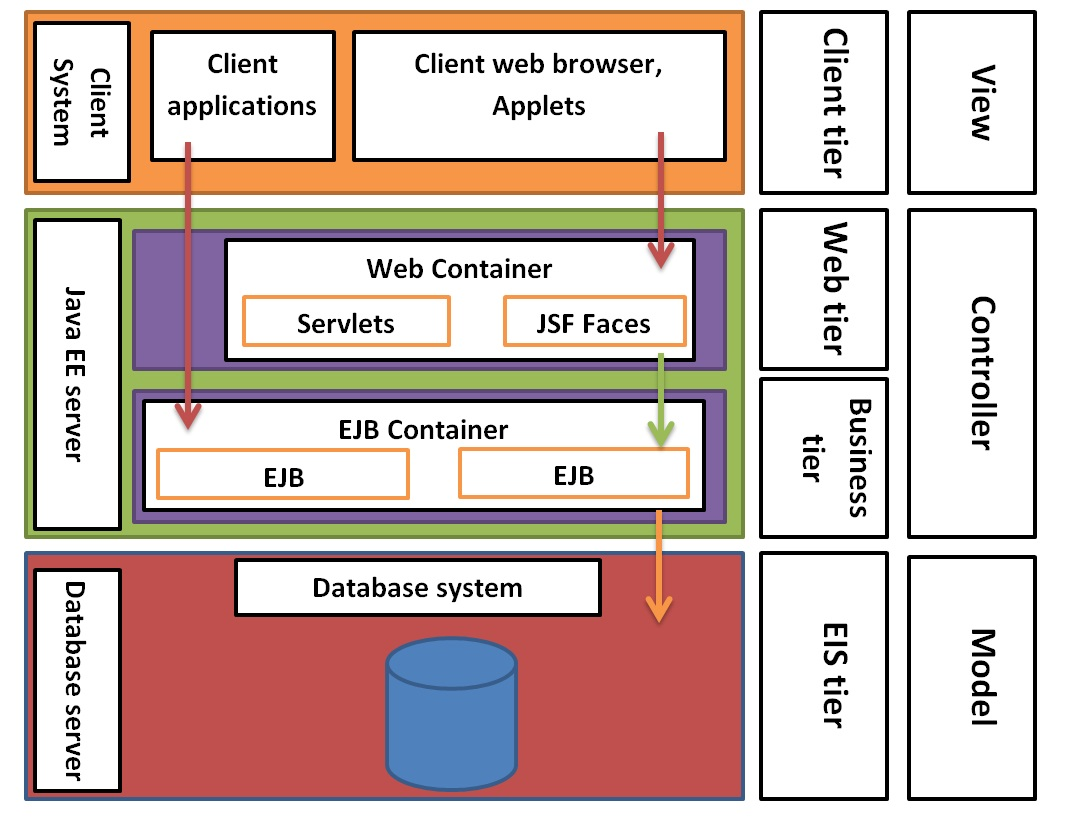
\includegraphics[scale=0.8]{../Images_Docs/Diagrams/Architecture/Java EE system architecture.jpg}
\caption{Java EE system architecture}
\end{figure}

\subsection{View}
The View component of the system architecture is used to represent and encapsulate the front-end of the system. It contains the client tier of the Java EE system architecture. Thus this allows the system to decouple the front-end and the back-end components. Allowing various clients to access the back-end without having to duplicate certain back-end tiers for each client. [Kayal, D., 2008]
\subsubsection{Client Tier}
This tier runs on the client system and encapsulates the various components that a client system may use to access the Java EE server-side tiers. These components include dynamic web pages, Java applications and Java applets. In order to make the Post-doctoral application management system accessible to any stakeholder over the internet and provide a uniform user experience the system will only make use of the dynamic web pages component provided by the Java EE client tier. [Oracle, 2014]  
\subsection{Controller}
The controller component of the system architecture is used to provide the business logic and manage and manipulate the view's request in order to provide communication between the Model component and the View. This component therefore hosts the web tier and the business tier of the Java EE application. This component is located on the Java EE server which is a multi-threaded application server. [Kayal, D., 2008] [Oracle, 2014] 
\subsubsection{Web Tier}
This Tier runs on the Java EE server and hosts the Web container. It provides the management and web page generation support for the web pages that the system has to provide to the view through the user of servlets, Java ServerPages and Java ServerFaces Facelets. Facilitates the communication between the business tier and client tier for web browser clients and applets. Client applications do not have to make use of the Web Tier and can directly skip to the business tier. But as stipulated above the other types of client components will not be considered for the project. [Oracle, 2014]
\subsubsection{Business Tier}
This Tier also runs on the Java EE server and hosts the Enterprise Java Bean container. It provides the business logic section for the Java EE application in the form of Enterprise Java Beans which are simply classes that represent various persistence entities of the data base, system messages, sessions, etc. This tier communicates with EIS tier in order to get access the database and various other lower level infrastructures that the Java EE application requires. [Oracle, 2014]
% More bullshit goes here.
\subsection{Model}
The Model component of the system architecture contains the various persistence storage infrastructure and lower level system management features such as transaction processing. It hosts the Enterprise Information System tier of the Java EE application. [Kayal, D., 2008]
\subsubsection{Enterprise Information Tier} 
The EIS tier provides mainly the support for database systems that is used by the Java-EE application. This tier can run on the Java-EE server as a virtual server or on a physically different database server. Due to the project budget and technical constraints the former will used by the system. [Oracle, 2014] 
 
%%%%%%%%%%%%%%%%%%%%%%%%%%%%%%%%%%%%%%%%%%%%%%%%%%%%%%%%%%%%%%%%%%%%%%%%%%%%%%%%%%%%%%%%%%%%%%%%%%%%%%%%%%%%%
\section{Architectural Tactics and Strategies} % skipped till further notice.
This section describes the architectural techniques which will be used in order for the system to satisfy the quality requirements. 

% This section needs a lot of paraphrasing...
\subsection{Concurrency}
The Java Platform has always offered support for concurrent programming, which is the basis for implementing many of the services offered by Java EE containers. This is realized through the two main concepts of having a multiple threads execute under a single process, in the case of Java EE mulitple beans execute under the JVM. The number of threads that can execute under the JVM can go well beyond thousands depending on factors such as the machine the JVM is running on and how it has been configured.\\

Even though the concurrent threads will mean better performance and a scalable implementation for the system they may lead to issues that effect the reliability and integrity of the system such as:
\begin{itemize}
\item Deadlocks,
\item Thread Starvation,
\item Concurrent  accessing of shared resources, and
\item Situations where the program generates incorrect data.
\end{itemize}

To deal with these issues Java EE provides concurrent utilities that access concurrent resources via JNDI lookup or resource injection. The components in the utilities ensure that the issues mentioned above are nullified. The primary components of interest in the concurrent utilities for our system are:
\begin{itemize}
\item managed executor service, 
\item managed scheduled executor service, 
\item managed thread factory, and 
\item context service.
\end{itemize}
\subsubsection{Concurrency Utilities for Java EE}
\subsubsection{Managed Executor Service}
A managed executor service is used by applications to execute submitted tasks asynchronously. Tasks are executed on threads that are
started and managed by the container. The context of the container is propagated to the thread executing the task.

For example, by using an ManagedExecutorService.submit() call, a task, such as the GenerateReportTask, could be submitted to execute at a later time and then, by using the Future object callback, retrieve the result when it becomes available ().

\subsubsection{Managed Scheduled Executor Service}
A managed scheduled executor service is used by applications to execute submitted tasks asynchronously at specific times. Tasks are executed on threads that are started and managed by the container. The context of the container is propagated to the thread executing the task. The API
provides the scheduling functionality that allows users to set a specific date/time for the Task execution programmatically in the application.

\subsubsection{Managed Thread Factory}
A managed thread factory is used by applications to create managed threads. The threads are started and managed by the container. The context of the container is propagated to the thread executing the task. This object can also be used to provide custom factories for specific use cases (with custom Threads) and, for example, set specific/proprietary properties to these objects (Cervera-Navarro, Evans, Jendrock, Haase and Markito 2014).

\subsection{Design Patterns}
\subsubsection{Builder Pattern}
The Builder Design Pattern allows for the construction of complex structures in small steps. An example of how it is used is in the process of making an application, the different elements of an application are separated. The process of creating objects speeds up as well. This construction of objects in small steps decreasing coupling and makes the code more testable. The design helps improve the flexibility as well as the maintainability of the code.  

\subsubsection{Factory Design Pattern}
The Factory Design Pattern provides centralised to create our Database entities and entries in an orderly fashion. The pattern allows the developers to define an interface for creating an object, but let the classes that implement the interface decide which class to instantiate. By doing this the code is now flexible and creation of new objects is much simpler. It also helps redundancy 

\subsubsection{State Design Pattern}
The State Design Pattern is best used in situations where the actions take place in a pre-defined order as with this project. The State pattern changes the state of the objects depending on how far in the pipeline. It provides a simple and clean way to change the state of an object during run time. The design pattern improves the usability of the system as users will know exactly when some change has taken place. 

\subsubsection{Dependency Injection}
This is used to implement, inversion control. The client is only allowed to use a service rather than creating their own services. The design pattern allows a client to remove all knowledge of a concrete implementation that it needs to use. This helps isolate the client from the impact of design changes and defects. It promotes re-usability, testability and maintainability 

\subsubsection{Database Access Objects}
The Database Access Object is used by all the application calls to provide specific data operations without exposing details of the database to external objects. It forms part of the Core J2EE Patterns. This design pattern acts an intermediary between the application and database, by moving back and forth between objects and database records. It also contains the effects of any changes to the persistence mechanism to a confined area and not the whole application. This pattern improves the audit-ability as well maintaining the integrity of the data contained in the system. 

The use of DAO will help reduce the existance of object-relational impedance mismatch present in the system. It will also contribute to the flexibilty of the system. In the case where the systems underlying persistance mechanism has to change only the DAO will have to be updated and all the places in the system where the DAO was used will then remain constant.

%%%%%%%%%%%%%%%%%%%%%%%%%%%%%%%%%%%%%%%%%%%%%%%%%%%%%%%%%%%%%%%%%%%%%%%%%%%%%%%%%%%%%%%%%%%%%%%%%%%%%%%%%%%%%
\section{Use of Reference Architecture and Framework}
The core design philosophy of the Java-EE platform is to provide a Java-EE application developer with a set of test and well maintained and reusable APIs as well as frameworks that allow them to focus rather on implementing the actual business logic and UI than focusing on the underlying system technical and management services such as authentication, session management, etc. Thus the Java EE platform provides a runtime environment for developing and running large-scale, multi-tiered, scalable, reliable, and secure network applications. As seen above it also provides a system architecture and various frameworks, discussed below, for implementing services for multi-tier applications that deliver the scalability, accessibility, and manageability needed by a system. Taking all the above into consideration this makes it ideal for the development of the project.

\subsection{JavaServer Faces (JSF)}
JSF is a web application GUI framework that is based on the JSP, EL and servlet technology that Java-EE provides. It allows the generation of various mark-up languages, such as HTML 4.0.1 and HTML 5, directly from objects and ORM model objects used by the Java-EE application. Thus it is ideal for system as the system needs to provide support for both HTML 5 and 4.0.1 web content.\\

It will help achieve the usability quality requirement as it will implement all aspects of the user interface.

\subsection{Java Persistence API}
Java EE is based on Java which is an object-oriented language. Whereas most modern day database management systems, DBMSs, provide relation databases. Thus to bridge this gap the Java Persistence API is used. It provides a Object Relational Mapping solution which allows the relation database to be viewed as a object-oriented database. Thus this critical for the system SoftServe wishes to develop as the system will make use of MySQL which is a relation database management system. The Java persistence API contains the following components:  
\begin{itemize}
\item Persistence API
\item The query language
\item ORM
\end{itemize}
\subsection{Java API for RESTful Web Services (JAX-RS)}
The JAX-RS API provides a way for the Java-EE application to provide web services or data transfer via the HTTP or HTTPS protocol using the Representational State Transfer, REST, architectural style. This accomplished by the user of various JAX-RS runtime annotations. This will allow the system to provide a set of lightweight web services to various clients across the internet. This will allow the system to easily be accesses by mobile and computer platforms alike and also be accessible over most companies firewalls as it will make use of the HTTPS protocol. Further this will allow for future expansion if client wishes it. To insure security a the POST command will be preferred above GET.[Cervera-Navarro, Evans, Jendrock, Haase and Markito, 2014]
\subsection{JUnit}
JUnit is a simple unit testing framework used to write repeatable tests. Test methods must be annotated by the @Test annotation. It is also possible to define a method to execute before (or after) each (or all) of the test methods with the @Before (or @After) and @BeforeClass (or @AfterClass) annotations. \\

It will be used to achieve the testbility of the system.
%\subsubsection{Java EE Connector Architecture}
%%%%%%%%%%%%%%%%%%%%%%%%%%%%%%%%%%%%%%%%%%%%%%%%%%%%%%%%%%%%%%%%%%%%%%%%%%%%%%%%%%%%%%%%%%%%%%%%%%%%%%%%%%%%%

\section{Access and Integration channels}
This section discusses the requirements for the access channels through which the system can be accessed by humans and other systems. Also it discusses the integration channels which need to be used by the system. 

\subsection{Access Channels}
To provide a system that is as accessible as possible the system provide its services through this essentially makes the system OS independent and accessible over firewalls since it will make use of the HTTPS protocol that is usually not blocked by firewalls. This also improves the usability the system as most computer user or mobile users are aware of how to use web browsers. The system will support the following versions of modern web browsers for both their computer and mobile counterparts:
\begin{enumerate}
\item Mozilla Firefox 20+
\item Google Chrome 30+
\item Microsoft Internet Explorer 9+
\item Apple Safari
\item Opera
\end{enumerate}

\subsection{Integration Channels}
As mentioned in the architecture requirements specification document the IT department of the University of Pretoria will only be willing to provide the SoftServe group with the knowledge of the Peoplesoft system in order to integrate it. Thus the SoftServe group will attempt to accommodate the PeopleSoft system as much as possible by conforming to same user name styling, export of data to formats that are used by the Peoplesoft system to import data. Also the since Peoplesoft is an Oracle enterprise system it would have been developed using Java-EE and the Java programming language. This is therefore a strong motivation for Java-EE to be used by the SoftServe group as a development platform for the system. So to allow integration at a more technical level. Though if the integration was to be done this would be done via the EIS teir using the Java EE Connector Architecture API and the JAX-WS API.  


%Upon successful complementation the system must be integrated able with the University of Pretoria's PeopleSoft system. Therefore it is sensible to implement the system in Java EE as it is one of the many components that form part of the multiple tiers that build up  PeopleSoft. \\

%The use of build tools such as Maven will provide a central piece of information with regards to the projects build, reporting and documentation. This central point of information will assist in the integration phase since it is implemented through a standardised build approach which can come into play at a later time through the use of EAI.\\

%The EAI will be achieved via  the logical integration architecture of Direct point-to-point integration (Kang, 2002). This means that the application management system will make direct JDBC calls to the universities databases tables (which needed to be setup to cater for our system at that point). The Integration method will be pushed-based data-level integration (or if all else fails UI-Level integration).
% http://www.javaworld.com/article/2074488/enterprise-java/enterprise-application-integration-using-j2ee.html

\section{Technologies}
This section discusses and elaborates on the technologies that the system will use and should also be seen as an extension of the architectural constraints, specified in the Architecture requirements specification document, in terms of elaboration.

\subsection{Integrated Development Environment}
The system should be buildable independent of an IDE but it will be developed on Netbeans 8.0 to allow for uniformity amongst the development team, with regards to coding style, and provide easy integration with the tools that will be used such as Javadoc, to generate  API documentation in HTML format.

\subsection{Build Tools}
\begin{itemize}
\item \textbf{Apache Maven} - This build tool was chosen due to the flexibility and power of it in terms of configurations, dependencies management, its ability to automate tests and the fact the project can easily be ported over to other IDEs such as the Netbeans IDE or even no IDE. 
\end{itemize}

\subsection{Server Operating System}

The system will be deployed on a single OS but will have clients that will use a variety of OSs. This is one of the main reasons the why the application's UI must be web browser based so to allow OS independent support. Thus the only prerequisite of the client's OS is that it needs to support a HTML 4 or 5 web browser and be internet accessible.
\begin{itemize}
\item \textbf{Server OS:}
	\begin{enumerate}
		\item Linux: Kubuntu 13.10
	\end{enumerate}
\item \textbf{Client OSs}
	\begin{enumerate}
		\item Windows: All
		\item Linux: All
		\item iOS: All
		\item Android: All
	\end{enumerate}
\end{itemize}

\subsection{Development technologies}
\subsubsection{Java Servlet Technology}
\textbf{Description}\\
A Java servlet is used to extend the Java-EE application server to support HTTP or HTTPS requests and responses. It allows the server to provide RESTful based web services to connecting clients. Thus it acts as a middle man between any HTTP or HTTPS client and the business tier. This will not be used directly but will be used the JSF framework.\\\\
\textbf{Reasons for use}\\
The JSF framework uses servlets to render JSF pages to HTML and provide them to clients connecting via HTTP or HTTPS. Secondly this will allow the solution to provide lightweight RESTful based web services that will help improve accessibility and availability of the solution. Further it will allow the solution to satisfy the access channel requirements.

\subsubsection{JavaServer Pages (JSP)}
\textbf{Description}\\
JSP is a technology that is used by the Java-EE platform to provide a native language approach to creating web pages. It uses HTML or XML to specify static content on a web page and Expression Language (EL) to provide dynamic content. This will not be used directly but will be used by the JSF framework.\\\\
\textbf{Reasons for use}\\
JSF pages is the a specialised version of JSP pages thus it is used in the JSF framework. Secondly it will help with the maintainability of the code as pages based on JSP technology are easily understandable and readable due to the simplicity of the HTML and XML mark-up languages.    
 
\subsubsection{Expression Language (EL)}
\textbf{Description}\\
It is a language used by JSP and JSF pages to write servlet based code snippets which allow the usage of the data available to the servlet to do calculations, call functions, get or set data. The language closely resembles the Java Language syntax.\\\\
\textbf{Reasons for use}\\
It is used by the JSP technology and JSF framework for dynamic content specification and communication with the backing servlet.

\subsubsection{JavaMail API}
\textbf{Description}\\
The JavaMail API provides a robust and well tested email communication infrastructure for any Java based applications.\\\\
\textbf{Reasons for use}\\
This technology will be employed by the system in order to provide the functional email notification infrastructure requirement needed by the solution.

\subsubsection{JavaBeans Activation Framework (JAF)}
\textbf{Description}\\
The JavaBeans Activation Framework allows the Java-EE application to determine the data type of some section of data and thus allow the application to provide access to it by encapsulating it and determining the operations that the application may perform on it.\\\\
\textbf{Reasons for use}\\
This technology is used by the JavaMail API thus it will be used by the system. 

\subsubsection{Java Database Connectivity API (JDBC)}
\textbf{Description}\\
The Java Database Connectivity API provides the a Java-EE application with the means to access data from various datasources including databases, spreadsheet, etc via the Java programming language.\\\\
\textbf{Reasons for use}\\
The system will use this to communicate with the databases located in the EIS tier of the system in order to retrieve and store data in the databases. 

\subsubsection{Java Transaction API (JTA)}
\textbf{Description}\\
The Java Transaction API provides the Java-EE Application with the means to handle and demarcate data transactions to the database. The API allows the the manual or automatic demarcation of database transactions and ensures that the database and ORM entities are synchronised after commits.\\\\ 
\textbf{Reasons for use}\\
This will be used in the system to improve the centralisation and accuracy of the data accessed by users. Further it will be used to allow access to multiple databases located in the EIS tier and the controlling of such resources.

\subsubsection{Enterprise JavaBeans (EJB)}
\textbf{Description}\\
The Enterprise JavaBeans is a component used by all Java-EE applications to encapsulate the various business logic of the application into reusable modules. Thus it contains the attributes and methods associated with the business logic module and hence can be treated as an stand alone unit that can be reused. The two primary EJBs are Session beans that represent a clients session and the data associated with it and a Message-driven bean that can a allow the component to receive messages asynchronously via event listeners. The system will make use of Stateless session EJBs in order to capture the back end services of the solution.\\\\
\textbf{Reasons for use}\\
The use of EJBs will ensure the modularity of the system and the re-usability of its components. Also within the Java-EE framework it is considered the core of the business tier and thus will be required.
  

\subsubsection{Java Naming and Directory Interface (JNDI)}
\textbf{Description}\\
The Java Naming and Directory Interface provides Java-EE applications with the ability to search for data across LDAP, DNS, etc, directory services. Above this it also allows the application to search for objects that exist within the application and provides access to them so that they can be used by the application. It is also used by Java-EE applications to locate object instances of EJBs and managed beans for usage by the application.\\\\
\textbf{Reasons for use}\\
This technology is a core service required by Java-EE applications to function and thus is needed by the solution.

\subsubsection{Java Architecture for XML Binding (JAXB)}
\textbf{Description}\\
JAXB is used to parse any XML data into a set of XML usable Java object instances that represent the content of the XML data. Likewise it is used to convert such objects to XML formatted data. This is accomplished by using an XML schema to define the structure or annotated classes.\\\\
\textbf{Reasons for use}\\
This will be used by the system to handle any XML data extraction or creation from or for storage.

\subsubsection{Jasper Reports}
\textbf{Description}\\
The Jasper reporting library provides a flexible, well-tested and maintained reporting framework to create reports based on data that is located in various data sources.\\\\
\textbf{Reasons for use}\\
This will be used to provide a reporting infrastructure as need by the system on a functional requirement level.   

\subsubsection{JSF Managed Beans}
\textbf{Description}\\
This is a standard POJO (Plain Old Java Object), which is used to provide encapsulated services to  front-end JSF pages. JSF access them via Expression Lanaguage. These beans can be used in conjunction with EJBs and CDI to communicate with the database or call back-end services of hosted by the server.\\\\
\textbf{Reasons for use}\\
This technology is part of the JSF framework and is therefore required. It further also allows improved modularity and re-usability of components.

\subsubsection{Primefaces}
\textbf{Description}\\
This is component library which is used to expand and provide an improved range of easy to use components for JSF pages. It incorporates Javascript, jQuery and AJAX in order to provide the various components.\\\\
\textbf{Reasons for use}\\
It is an easy to use, versatile library that allows the solution provide a sophisticated and clean user interface. Further is highly compatible with mobile platform HTTP web browsers thus allowing the solution to provide better accessibility without extensive modification.    

\subsubsection{Mockito}
\textbf{Description}\\
This is a mock framework that allows the mocking of dependencies during unit testing phases.\\\\
\textbf{Reasons for use}\\
It is easy to use and provides a great number of effective features that will help enhance unit testing during the development of the solution. Thus it helps improve the testability of the solution.

\subsubsection{MySQL DBMS}
\textbf{Description}\\
This is a well-proven open-source relational database management system that provides extensive set of features for maintaining the data and database.\\\\
\textbf{Reasons for use}\\
It a is well-proven DBMS. Further since the data captured by the solution will fit well in a relation approach the DBMS will be efficient enough to meet the performance and scalability requirements of the solution.



\newpage


\newpage
\section{Glossary:}
\vspace{0.2in}

\begin{itemize}

\item \textbf{API} - Application Programming Interface
\item \textbf{Application} -Both renewal applications or new fellowship applications are seen as applications by this project.
\item \textbf{CV} - Curriculum Vita
\item \textbf{EAI} - Enterprise Application Integration
\item \textbf{NRF} - National Research Foundation
\item \textbf{Spreadsheet} - A special type of computer document that is used to represent data in rows and columns.
\item \textbf{GlassFish} - GlassFish is a web server software package that is very flexible and compatible with Java EE applications. 
\item \textbf{HTML} - Hyper Text Mark-up Language
\item \textbf{HTTPS} - Hyper Text Transfer Protocol Secure is a higher level network oriented communication rule set that is highly secure and is used by all web browsers. 
\item \textbf{Java EE} - Java Enterprise Edition
\item \textbf{MySQL} - Is a relational persistence database package that provides all the necessary management tools to run and manage a database server.
\item \textbf{Object-Oriented} - A programming language style that encapsulates everything as an object instance of a particular class of attributes and methods.
\item \textbf{JDBC} - Java Database Connection
\item \textbf{MVC} - Model View Controller
\item \textbf{UI} - User Interface
\item \textbf{UP} - University of Pretoria
\item \textbf{Application} - Both a renewal and new fellowship are seen as applications.

\end{itemize}	


\vspace{0.5in}


\end{document}